\section{Utente Autenticato}

Di seguito vengono elencati i casi d'uso per l'utente autenticato.
\subsection{Casi d'Uso}

\subsubsection{UC-U8}

    \begin{figure}[H]
      \begin{center}
        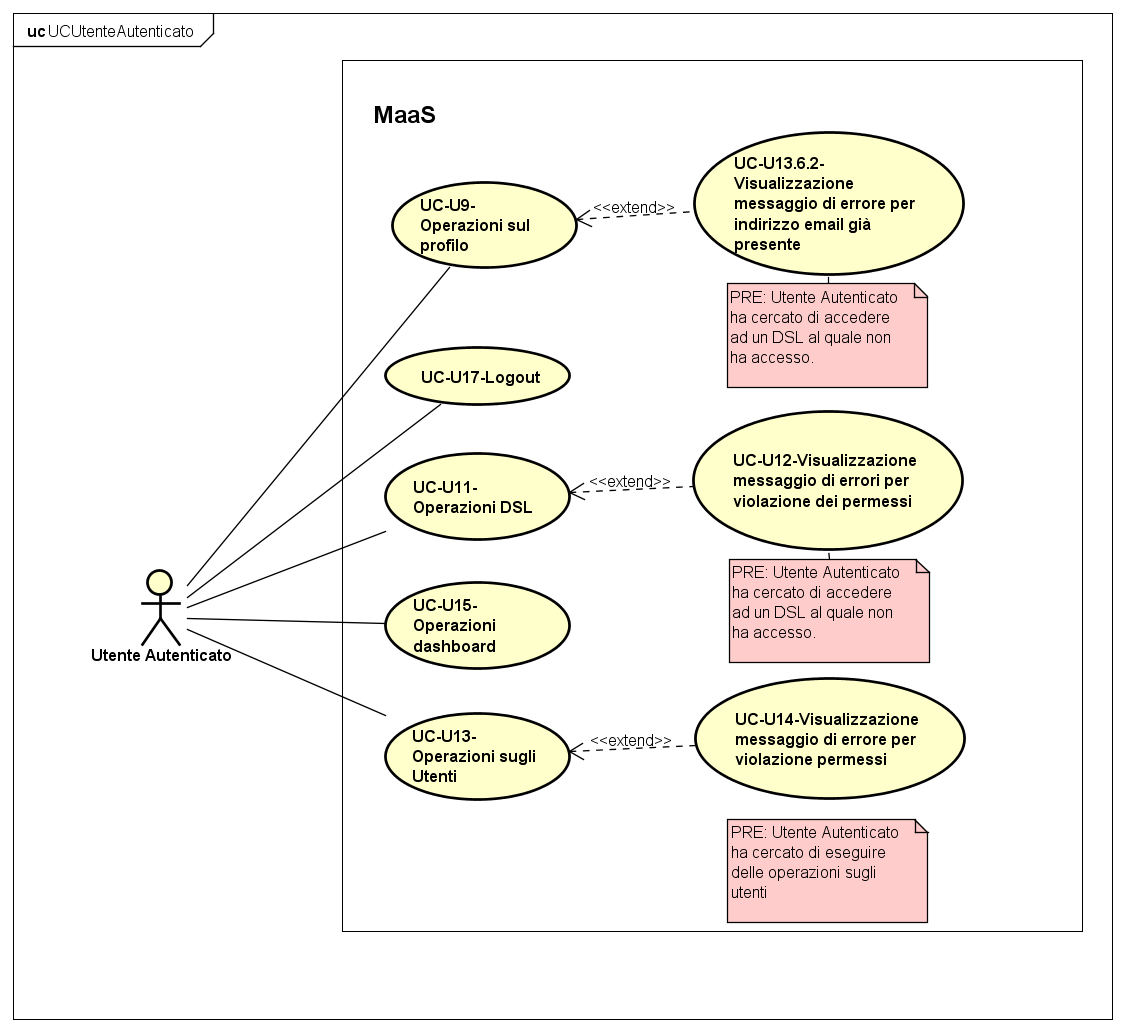
\includegraphics[width=12cm]{res/img/UCUtenti/UCUtenteA/UC-U8-OperazioniUtenteAutenticato}
      \caption{UC-U8 - Operazioni dell'utente autenticato}
      \end{center} 
    \end{figure}    
    
    %Tabella 
    \begin{center}
      \bgroup
      \def\arraystretch{1.8}     
      \begin{longtable}{  p{3.5cm} | p{8cm} } 
        
        \hline
        \multicolumn{2}{ | c | }{ \cellcolor[gray]{0.9} \textbf{UC-U8 - Operazioni dell'utente autenticato}} \\ 
        \hline
        
        \textbf{Attori Primari} & Utente autenticato \\ 
        \textbf{Scopo e Descrizione} & L’utente autenticato può: modificare il proprio profilo, effettuare delle operazioni nella pagina Dashboard, effettuare delle operazioni di creazione/modifica/esecuzione del DSL (a seconda dei suoi permessi) e gestire altri utenti (quest'ultima funzionalità è riservata ad un ruolo superiore o uguale all'admin). \\ 
        
        \textbf{Precondizioni}  & L’applicazione MaaS è funzionante e pronta all'uso. L'utente autenticato può accedere alla propria pagina Dashboard. \\ 
        
        \textbf{Postcondizioni} & L'applicazione ha eseguito le azioni richieste dall'utente. \\ 
        \textbf{Flusso Principale} & 1. L'utente modifica il proprio profilo (UC-U9)
        
2. L'utente effettua delle operazioni nella pagina Dashboard (UC-U15)

3. L'utente effettua delle operazioni di creazione/modifica/esecuzione del DSL (a seconda dei suoi permessi) (UC-U11)

4. L'utente gestisce altri utenti (quest'ultima funzionalità è riservata ad un ruolo superiore o uguale all'admin) (UC-U13) \\
        \textbf{Estensioni} & 1. L'utente autenticato visualizza un messaggio di errore nella proceduro di modifica del profilo dovuto all'inserimento di un indirizzo email già presente (UC-U13.6.2)
        
2. L'utente autenticato visualizza un messaggio di errore durante le operazioni effettuate sul DSL dovuto alla violazione dei permessi (UC-U12)

3. L'utente autenticato visualizza un messaggio di errore durante le operazioni sugli utenti dovute alla violazione dei permessi (UC-u14) \\
        \textbf{Inclusioni} & Nessuna \\
      \end{longtable}
      \egroup
    \end{center} 


\subsubsection{UC-U9}

    \begin{figure}[H]
      \begin{center}
        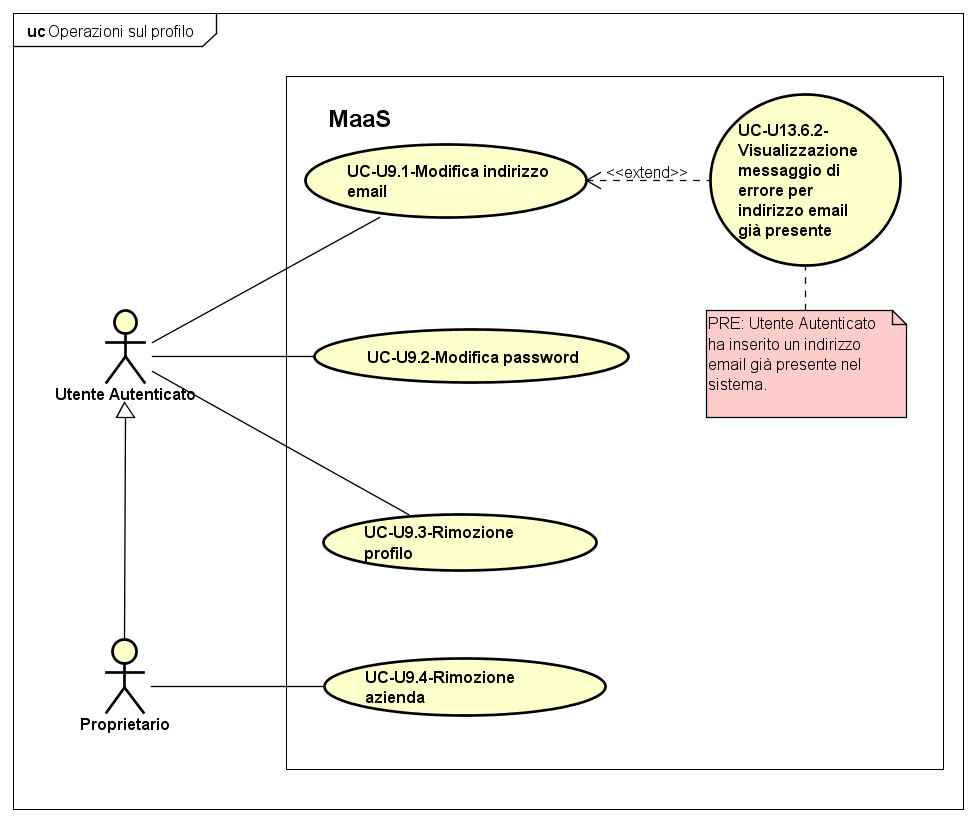
\includegraphics[width=12cm]{res/img/UCUtenti/UCUtenteA/UC-U9- Operazioni sul profilo/Operazioni sul profilo}
      \caption{UC-U9 - Operazioni sul profilo}
      \end{center} 
    \end{figure}    
    
    %Tabella 
    \begin{center}
      \bgroup
      \def\arraystretch{1.8}     
      \begin{longtable}{  p{3.5cm} | p{8cm} } 
        
        \hline
        \multicolumn{2}{ | c | }{ \cellcolor[gray]{0.9} \textbf{UC-U9 - Operazioni sul profilo}} \\ 
        \hline
        
        \textbf{Attori Primari} & Utente autenticato \\ 
        \textbf{Scopo e Descrizione} & L'utente autenticato visualizza la pagina per apportare modifiche al profilo personale. Può decidere di: modificare l'indirizzo email, la password, o rimuovere il profilo. \\ 
        
        \textbf{Precondizioni}  & L’applicazione MaaS è funzionante e pronta all'uso. L'utente autenticato può accedere alla propria pagina Dashboard. \\ 
        
        \textbf{Postcondizioni} & Le (eventuali) modifiche del profilo richieste dall'utente sono state apportate. \\ 
        \textbf{Flusso Principale} & 1. L'utente autenticato modifica il proprio indirizzo email (UC-U9.1)
        
2. L'utente autenticato modifica la propria password (UC-U9.2)

3. L'utente autenticato rimuove il suo profilo/account (UC-U9.3)

4. Il proprietario rimuove la propria azienda (UC-U9.4) \\
        \textbf{Estensioni} & 1. L'utente visualizza un messaggio di errore durante la modifica dell'email dovuto all'inserimento di un indirizzo email già presente. (UC-U13.6.2) \\
        \textbf{Inclusioni} & Nessuna \\
      \end{longtable}
      \egroup
    \end{center} 

\subsubsection{UC-U9.1}
 

    \begin{figure}[H]
      \begin{center}
        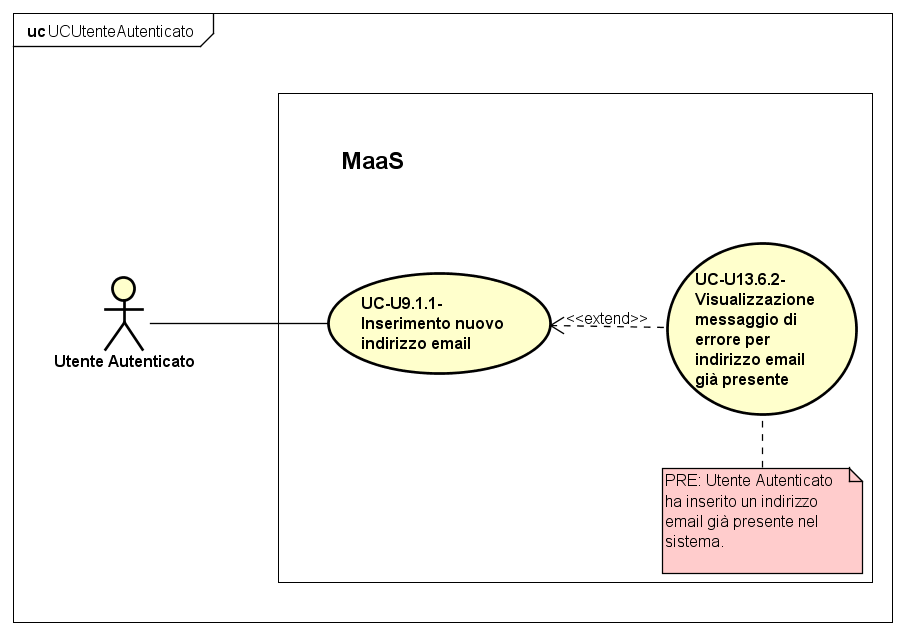
\includegraphics[width=12cm]{res/img/UCUtenti/UCUtenteA/UC-U9.1-Modifica indirizzo email/UC-U9.1-Modifica indirizzo email}
      \caption{UC-U9.1 - Modifica indirizzo email}
      \end{center} 
    \end{figure}

    %Tabella 
    \begin{center}
      \bgroup
      \def\arraystretch{1.8}     
      \begin{longtable}{  p{3.5cm} | p{8cm} } 
        
        \hline
        \multicolumn{2}{ | c | }{ \cellcolor[gray]{0.9} \textbf{UC-U9.1 - Modifica indirizzo email}} \\ 
        \hline
        
        \textbf{Attori Primari} & Utente autenticato \\ 
        \textbf{Scopo e Descrizione} & L'utente autenticato può modificare il proprio indirizzo email nella procedura di modifica del profilo. \\ 
        
        \textbf{Precondizioni}  & L'utente autenticato ha visualizzato la pagina di modifica del profilo. \\ 
        
        \textbf{Postcondizioni} & L'utente autenticato dispone di un nuovo indirizzo email, che sostituisce il vecchio. \\ 
        \textbf{Flusso Principale} & 1. L'utente autenticato inserisce un nuovo indirizzo email (UC-U9.1.1) \\
        \textbf{Estensioni} & 1. L'utente autenticato visualizza un messaggio di errore causato dall'inserimento di un indirizzo email già presente (UC-U13.6.2) \\
        \textbf{Inclusioni} & Nessuna
      \end{longtable}
      \egroup
    \end{center}
    
\subsubsection{UC-U9.1.1}

    %Tabella 
    \begin{center}
      \bgroup
      \def\arraystretch{1.8}     
      \begin{longtable}{  p{3.5cm} | p{8cm} } 
        
        \hline
        \multicolumn{2}{ | c | }{ \cellcolor[gray]{0.9} \textbf{UC-U9.1.1 - Inserimento di un nuovo indirizzo email}} \\ 
        \hline
        
        \textbf{Attori Primari} & Utente autenticato \\ 
        \textbf{Scopo e Descrizione} & L'utente autenticato può inserire un nuovo indirizzo email nella procedura di modifica del profilo. \\ 
        
        \textbf{Precondizioni}  & L'utente autenticato ha visualizzato la pagina di modifica del profilo. \\ 
        
        \textbf{Postcondizioni} & L'utente autenticato ha inserito un nuovo indirizzo email. \\ 
        \textbf{Flusso Principale} & Nessuno \\
        \textbf{Estensioni} & Nessuna \\
        \textbf{Inclusioni} & Nessuna
      \end{longtable}
      \egroup
    \end{center}
\subsubsection{UC-U9.2}
 

    \begin{figure}[H]
      \begin{center}
        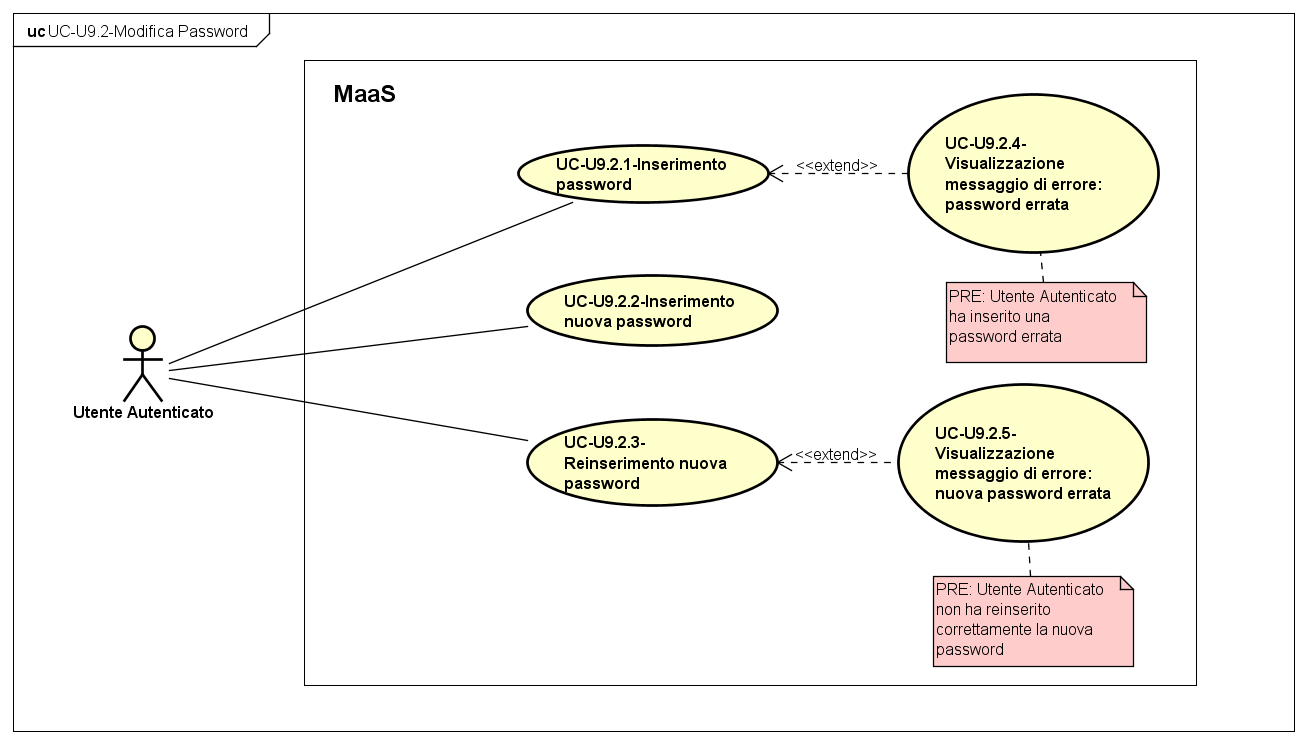
\includegraphics[width=12cm]{res/img/UCUtenti/UCUtenteA/UC-U9.2-Modifica password/UC-U9.2-Modifica password}
      \caption{UC-U9.2 - Modifica password}
      \end{center} 
    \end{figure}

    %Tabella 
    \begin{center}
      \bgroup
      \def\arraystretch{1.8}     
      \begin{longtable}{  p{3.5cm} | p{8cm} } 
        
        \hline
        \multicolumn{2}{ | c | }{ \cellcolor[gray]{0.9} \textbf{UC-U9.2 - Modifica password}} \\ 
        \hline
        
        \textbf{Attori Primari} & Utente autenticato \\ 
        \textbf{Scopo e Descrizione} & L'utente autenticato può modificare la password del proprio account. \\ 
        
        \textbf{Precondizioni}  & L'utente autenticato ha visualizzato la pagina di modifica del profilo. \\ 
        
        \textbf{Postcondizioni} & L'utente autenticato ha sostituito la password precedente con quella da lui inserita. \\ 
        \textbf{Flusso Principale} & 1. L'utente autenticato inserisce la password corrente (UC-U9.2.1)
        
2. L'utente autenticato inserisce una nuova password (UC-U9.2.2)

3. L'utente autenticato re-inserisce la nuova password (UC-U9.2.3) \\
        \textbf{Estensioni} & 1. L'utente autenticato visualizza un messaggio di errore dovuto all'inserimento di una password errata (UC-U9.2.4)
        
2. L'utente autenticato visualizza un messaggio di errore dovuto al reinserimento della nuova password (non corrisponde alla nuova password già inserita) (UC-U9.2.5) \\
        \textbf{Inclusioni} & Nessuna
      \end{longtable}
      \egroup
    \end{center}
    
\subsubsection{UC-U9.2.1}

    %Tabella 
    \begin{center}
      \bgroup
      \def\arraystretch{1.8}     
      \begin{longtable}{  p{3.5cm} | p{8cm} } 
        
        \hline
        \multicolumn{2}{ | c | }{ \cellcolor[gray]{0.9} \textbf{UC-U9.2.1 - Inserimento Password}} \\ 
        \hline
        
        \textbf{Attori Primari} & Utente autenticato \\ 
        \textbf{Scopo e Descrizione} & L'utente autenticato inserisce la propria password. \\ 
        
        \textbf{Precondizioni}  & L'utente autenticato ha visualizzato la pagina di modifica del profilo. \\ 
        
        \textbf{Postcondizioni} & L'utente autenticato ha inserito la propria password. \\ 
        \textbf{Flusso Principale} & Nessuno \\
        \textbf{Estensioni} & Nessuna \\
        \textbf{Inclusioni} & Nessuna
      \end{longtable}
      \egroup
    \end{center}
\subsubsection{UC-U9.2.2}

    %Tabella 
    \begin{center}
      \bgroup
      \def\arraystretch{1.8}     
      \begin{longtable}{  p{3.5cm} | p{8cm} } 
        
        \hline
        \multicolumn{2}{ | c | }{ \cellcolor[gray]{0.9} \textbf{UC-U9.2.2 - Inserimento nuova password}} \\ 
        \hline
        
        \textbf{Attori Primari} & Utente autenticato \\ 
        \textbf{Scopo e Descrizione} & L'utente autenticato inserisce una nuova password in sostituzione di quella precedente.  \\ 
        
        \textbf{Precondizioni}  & L'utente autenticato ha visualizzato la pagina di modifica del profilo. \\ 
        
        \textbf{Postcondizioni} & L'utente autenticato ha inserito una nuova password. \\ 
        \textbf{Flusso Principale} & Nessuno \\
        \textbf{Estensioni} & Nessuna \\
        \textbf{Inclusioni} & Nessuna
      \end{longtable}
      \egroup
    \end{center}
	
\subsubsection{UC-U9.2.3}

    %Tabella 
    \begin{center}
      \bgroup
      \def\arraystretch{1.8}     
      \begin{longtable}{  p{3.5cm} | p{8cm} } 
        
        \hline
        \multicolumn{2}{ | c | }{ \cellcolor[gray]{0.9} \textbf{UC-U9.2.3 - Reinserimento password}} \\ 
        \hline
        
        \textbf{Attori Primari} & Utente autenticato \\ 
        \textbf{Scopo e Descrizione} & L'utente autenticato ripete l'inserimento della nuova password. \\ 
        
        \textbf{Precondizioni}  & L'utente autenticato ha precedentemente inserito la nuova password. (UC-U9.2.2) \\ 
        
        \textbf{Postcondizioni} & L'utente autenticato ha completato la procedura di cambiamento della password. La nuova password inserita ha sostituito la password precedente. \\ 
        \textbf{Flusso Principale} & Nessuno \\
        \textbf{Estensioni} & Nessuna \\
        \textbf{Inclusioni} & Nessuna
      \end{longtable}
      \egroup
    \end{center}
	
\subsubsection{UC-U9.2.4}

    %Tabella 
    \begin{center}
      \bgroup
      \def\arraystretch{1.8}     
      \begin{longtable}{  p{3.5cm} | p{8cm} } 
        
        \hline
        \multicolumn{2}{ | c | }{ \cellcolor[gray]{0.9} \textbf{UC-U9.2.4 - Visualizzazione messaggio di errore: password errata}} \\ 
        \hline
        
        \textbf{Attori Primari} & Utente autenticato \\ 
        \textbf{Scopo e Descrizione} & L'utente autenticato visualizza un messaggio di errore durante procedura di modifica del profilo dovuto all'inserimento di una password errata. \\ 
        
        \textbf{Precondizioni}  & L'utente autenticato ha inserito una password errata nella procedura di cambio della password. \\ 
        
        \textbf{Postcondizioni} & L'utente autenticato ha visualizzato il messaggio di errore. \\ 
        \textbf{Flusso Principale} & Nessuno \\
        \textbf{Estensioni} & Nessuna \\
        \textbf{Inclusioni} & Nessuna
      \end{longtable}
      \egroup
    \end{center}

\subsubsection{UC-U9.2.5}

    %Tabella 
    \begin{center}
      \bgroup
      \def\arraystretch{1.8}     
      \begin{longtable}{  p{3.5cm} | p{8cm} } 
        
        \hline
        \multicolumn{2}{ | c | }{ \cellcolor[gray]{0.9} \textbf{UC-U9.2.5 - Visualizzazione messaggio di errore: nuova password errata}} \\ 
        \hline
        
        \textbf{Attori Primari} & Utente autenticato \\ 
        \textbf{Scopo e Descrizione} & L'utente autenticato visualizza un messaggio di errore dovuto al reinserimento errato della nuova password (la nuova password è diversa da quella inserita la prima volta). \\ 
        
        \textbf{Precondizioni}  & L'utente autenticato non ha reinserito correttamente la nuova password. \\ 
        
        \textbf{Postcondizioni} & L'utente autenticato ha visualizzato il messaggio di errore. \\ 
        \textbf{Flusso Principale} & Nessuno \\
        \textbf{Estensioni} & Nessuna \\
        \textbf{Inclusioni} & Nessuna
      \end{longtable}
      \egroup
    \end{center}
\subsubsection{UC-U9.3}

    %Tabella 
    \begin{center}
      \bgroup
      \def\arraystretch{1.8}     
      \begin{longtable}{  p{3.5cm} | p{8cm} } 
        
        \hline
        \multicolumn{2}{ | c | }{ \cellcolor[gray]{0.9} \textbf{UC-U9.3 - Rimozione profilo}} \\ 
        \hline
        
        \textbf{Attori Primari} & Utente autenticato \\ 
        \textbf{Scopo e Descrizione} & L'utente autenticato deccide di rimuovere il suo profilo da MaaS. \\ 
        
        \textbf{Precondizioni}  & L'utente autenticato ha acconsentito con la continuazione della procedura. \\ 
        
        \textbf{Postcondizioni} & L'utente autenticato visualizza un messaggio di avvenuta cancellazione e le sue credenziali vengono eliminate da MaaS. \\ 
        \textbf{Flusso Principale} & Nessuno \\
        \textbf{Estensioni} & Nessuna \\
        \textbf{Inclusioni} & Nessuna
      \end{longtable}
      \egroup
    \end{center}
\subsubsection{UC-U9.4}

    %Tabella 
    \begin{center}
      \bgroup
      \def\arraystretch{1.8}     
      \begin{longtable}{  p{3.5cm} | p{8cm} } 
        
        \hline
        \multicolumn{2}{ | c | }{ \cellcolor[gray]{0.9} \textbf{UC-U9.4 - Rimozione azienda}} \\ 
        \hline
        
        \textbf{Attori Primari} & Proprietario \\ 
        \textbf{Scopo e Descrizione} & Il proprietario decide di rimuovere l'azienda con tutte le sue informazioni e i suoi utenti da MaaS. \\ 
        
        \textbf{Precondizioni}  & Il proprietario ha acconsentito con la continuazione della procedura. \\ 
        
        \textbf{Postcondizioni} & Il proprietario visualizza un messaggio di avvenuta cancellazione e tutti i dati e gli utenti registrati nell'azienda vengono cancellati da MaaS. \\ 
        \textbf{Flusso Principale} & Nessuno \\
        \textbf{Estensioni} & Nessuna \\
        \textbf{Inclusioni} & Nessuna
      \end{longtable}
      \egroup
    \end{center}
\subsubsection{UC-U11}

        \begin{figure}[H]
          \begin{center}
            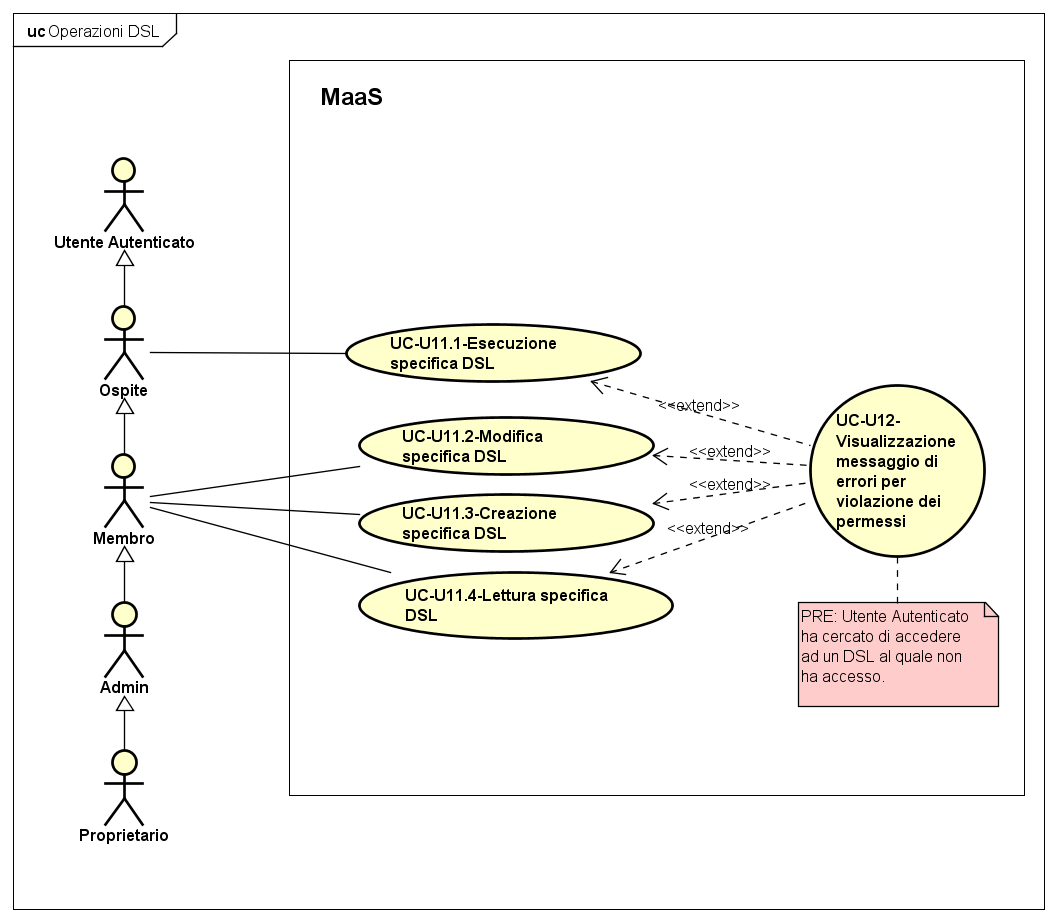
\includegraphics[width=12cm]{res/img/UCUtenti/UCUtenteA/UC-U11-Operazioni DSL/UC-U11-Operazioni DSL}
          \caption{UC-U11 - Operazioni DSL}
          \end{center} 
        \end{figure}
        
        %Tabella 
        \begin{center}
          \bgroup
          \def\arraystretch{1.8}     
          \begin{longtable}{  p{3.5cm} | p{8cm} } 
            
            \hline
            \multicolumn{2}{ | c | }{ \cellcolor[gray]{0.9} \textbf{UC-U11 - Operazioni DSL}} \\ 
            \hline
            
            \textbf{Attori Primari} & Utente Autenticato, Ospite, Membro, Admin, Proprietario \\ 
            \textbf{Scopo e Descrizione} & L’utente visualizza la pagina per apportare modifiche sulle DSL. Può decidere di: eseguire, modificare, creare e leggere una specifica DSL.\\ 
            
            \textbf{Precondizioni}  & L’applicazione MaaS è funzionante e pronta all'uso. Gli utenti possono accedere alla propria pagina Dashboard. \\ 
            
            \textbf{Postcondizioni} & Le (eventuali) modifiche sono state apportate. \\ 
            \textbf{Flusso Principale} & 1. L'Ospite, il Membro, l'Admin e il Proprietario possono eseguire una specifica DSL (UC-U11.1)  
            
            2. Il Membro, l'Admin e il Proprietario possono modificare una specifica DSL (UC-U11.2)
            
            3. Il Membro, l'Admin e il Proprietario possono creare una specifica DSL (UC-U11.3)
            
            4. Il Membro, l'Admin e il Proprietario possono leggere una specifica DSL (UC-U11.4)\\
            \textbf{Estensioni} & 1. L'utente visualizza un messaggio di errore in quanto non ha i permessi per operare sulla specifica DSL (UC-U12)  \\
            \textbf{Inclusioni} & Nessuna
          \end{longtable}
          \egroup
        \end{center}
\subsubsection{UC-U11.1}
                %Tabella 
                \begin{center}
                  \bgroup
                  \def\arraystretch{1.8}     
                  \begin{longtable}{  p{3.5cm} | p{8cm} } 
                    
                    \hline
                    \multicolumn{2}{ | c | }{ \cellcolor[gray]{0.9} \textbf{UC-U11.1 - Esecuzione specifica DSL}} \\ 
                    \hline
                    
                    \textbf{Attori Primari} & Utente Autenticato, Ospite, Membro, Admin, Proprietario  \\ 
                    \textbf{Scopo e Descrizione} & L'Utente Autenticato, Ospite, Membro, Admin, Proprietario eseguono una specifica DSL\\ 
                    
                    \textbf{Precondizioni}  & L’applicazione MaaS è funzionante e pronta all'uso. Gli utenti possono accedere alla propria pagina Dashboard.\\ 
                    
                    \textbf{Postcondizioni} & L'utente visualizza il risultato della DSL \\ 
                    \textbf{Flusso Principale} & Nessuno\\
                    \textbf{Estensioni} & 1. L'utente visualizza un messaggio di errore in quanto non ha i permessi per operare sulla specifica DSL (UC-U12)  \\
                    \textbf{Inclusioni} & Nessuna
                  \end{longtable}
                  \egroup
                \end{center}
\subsubsection{UC-U11.2}
                %Tabella 
                \begin{center}
                  \bgroup
                  \def\arraystretch{1.8}     
                  \begin{longtable}{  p{3.5cm} | p{8cm} } 
                    
                    \hline
                    \multicolumn{2}{ | c | }{ \cellcolor[gray]{0.9} \textbf{UC-U11.2 - Modifica specifica DSL}} \\ 
                    \hline
                    
                    \textbf{Attori Primari} & Membro, Admin, Proprietario  \\ 
                    \textbf{Scopo e Descrizione} & Il Membro, Admin, Proprietario modificano una specifica DSL tramite l'editor\\ 
                    
                    \textbf{Precondizioni}  & L’applicazione MaaS è funzionante e pronta all'uso. Gli utenti possono accedere alla propria pagina Dashboard. \\ 
                    
                    \textbf{Postcondizioni} & L'utente modifica la DSL \\ 
                    \textbf{Flusso Principale} & Nessuno\\
                    \textbf{Estensioni} & 1. L'utente visualizza un messaggio di errore in quanto non ha i permessi per operare sulla specifica DSL (UC-U12)  \\
                    \textbf{Inclusioni} & Nessuna
                  \end{longtable}
                  \egroup
                \end{center}
\subsubsection{UC-U11.3}
                %Tabella 
                \begin{center}
                  \bgroup
                  \def\arraystretch{1.8}     
                  \begin{longtable}{  p{3.5cm} | p{8cm} } 
                    
                    \hline
                    \multicolumn{2}{ | c | }{ \cellcolor[gray]{0.9} \textbf{UC-U11.3 - Creazione specifica DSL}} \\ 
                    \hline
                    
                    \textbf{Attori Primari} & Membro, Admin, Proprietario  \\ 
                    \textbf{Scopo e Descrizione} & Il Membro, Admin, Proprietario creano una specifica DSL tramite l'editor\\ 
                    
                    \textbf{Precondizioni}  & L’applicazione MaaS è funzionante e pronta all'uso. Gli utenti possono accedere alla propria pagina Dashboard.\\ 
                    
                    \textbf{Postcondizioni} & L'utente aggiunge la DSL a MaaS \\ 
                    \textbf{Flusso Principale} & Nessuno\\
                    \textbf{Estensioni} & 1. L'utente visualizza un messaggio di errore in quanto non ha i permessi per operare sulla specifica DSL (UC-U12)  \\
                    \textbf{Inclusioni} & Nessuna
                  \end{longtable}
                  \egroup
                \end{center}
\subsubsection{UC-U11.4}
                %Tabella 
                \begin{center}
                  \bgroup
                  \def\arraystretch{1.8}     
                  \begin{longtable}{  p{3.5cm} | p{8cm} } 
                    
                    \hline
                    \multicolumn{2}{ | c | }{ \cellcolor[gray]{0.9} \textbf{UC-U11.4 - Lettura specifica DSL}} \\ 
                    \hline
                    
                    \textbf{Attori Primari} & Membro, Admin, Proprietario  \\ 
                    \textbf{Scopo e Descrizione} & Il Membro, Admin, Proprietario leggono una specifica DSL\\ 
                    
                    \textbf{Precondizioni}  & L’applicazione MaaS è funzionante e pronta all'uso. Gli utenti possono accedere alla propria pagina Dashboard.\\ 
                    
                    \textbf{Postcondizioni} & L'utente legge la DSL \\ 
                    \textbf{Flusso Principale} & Nessuno\\
                    \textbf{Estensioni} & 1. L'utente visualizza un messaggio di errore in quanto non ha i permessi per operare sulla specifica DSL (UC-U12)  \\
                    \textbf{Inclusioni} & Nessuna
                  \end{longtable}
                  \egroup
                \end{center}
\subsubsection{UC-U12}
      
        %Tabella 
        \begin{center}
          \bgroup
          \def\arraystretch{1.8}     
          \begin{longtable}{  p{3.5cm} | p{8cm} } 
            
            \hline
            \multicolumn{2}{ | c | }{ \cellcolor[gray]{0.9} \textbf{UC-U12 - Visualizzazione di messaggio di errore per violazione dei permessi}} \\ 
            \hline
            
            \textbf{Attori Primari} & Utente autenticato \\ 
            \textbf{Scopo e Descrizione} & L’utente autenticato visualizza un messaggio di errore nel tentativo di eseguire un'operazione sul DSL.\\ 
            
            \textbf{Precondizioni}  & L'utente autenticato ha eseguito un'operazione sul DSL di cui non dispone i permessi. \\ 
            
            \textbf{Postcondizioni} & L'utente autenticato ha visualizzato il messaggio di errore. \\ 
            \textbf{Flusso Principale} & Nessuno \\
            \textbf{Estensioni} & Nessuna  \\
            \textbf{Inclusioni} & Nessuna
          \end{longtable}
          \egroup
        \end{center}
\subsubsection{UC-U13}

        \begin{figure}[H]
          \begin{center}
            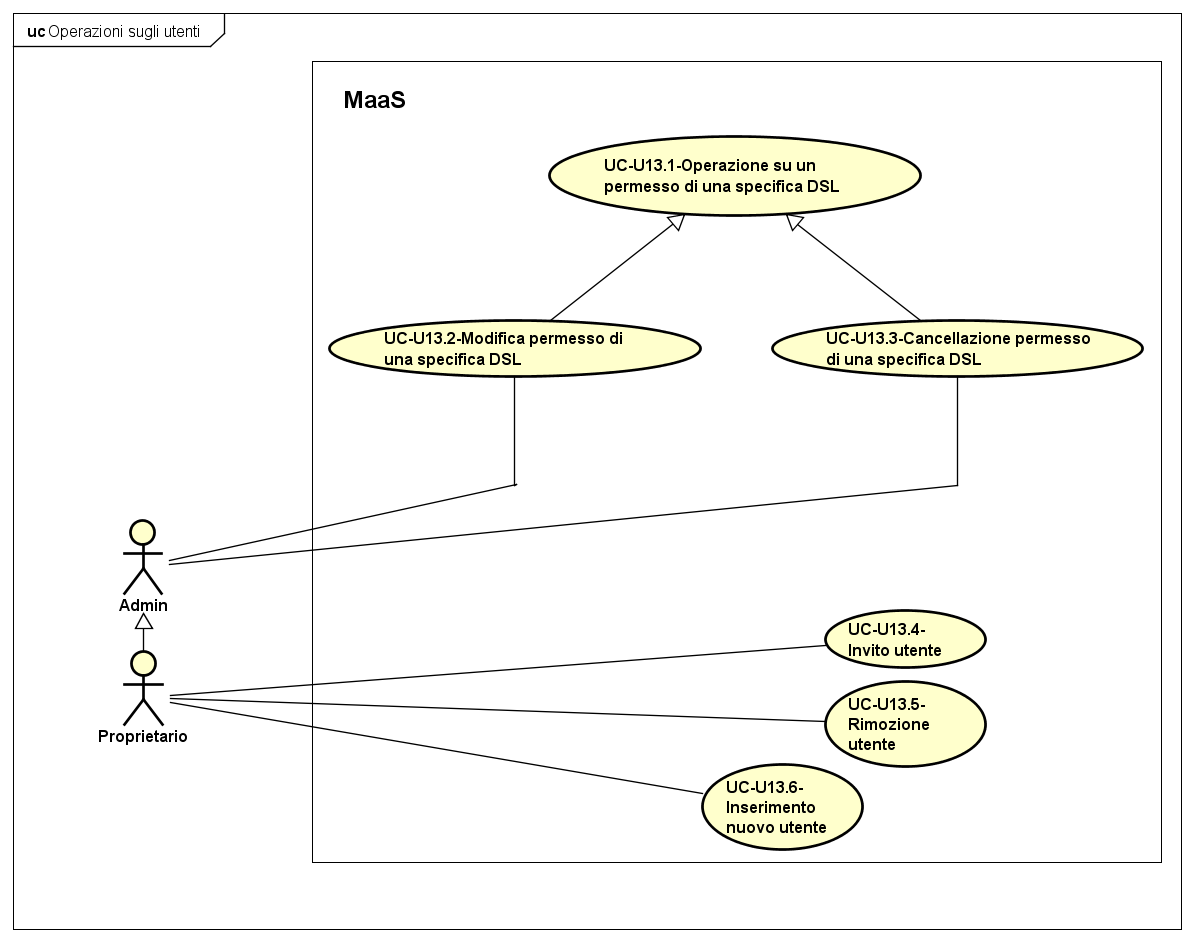
\includegraphics[width=12cm]{res/img/UCUtenti/UCUtenteA/UC-U13-Operazioni sugli Utenti/UC-U13-Operazioni sugli Utenti}
          \caption{UC-U13 - Operazioni sugli utenti}
          \end{center} 
        \end{figure}
        
        %Tabella 
        \begin{center}
          \bgroup
          \def\arraystretch{1.8}     
          \begin{longtable}{  p{3.5cm} | p{8cm} } 
            
            \hline
            \multicolumn{2}{ | c | }{ \cellcolor[gray]{0.9} \textbf{UC-U13 - Operazioni sugli utenti}} \\ 
            \hline
            
            \textbf{Attori Primari} & Amministratore, Proprietario \\ 
            \textbf{Scopo e Descrizione} & L'Amministratore e il Proprietario visualizzano la pagina per apportare modifiche sugli utenti. Possono decidere di: operare su una specifica DSL accedendo all'editor e inserire, rimuovere, invitare un nuovo utente.\\ 
            
            \textbf{Precondizioni}  & L'amministratore e il Proprietario dispongono dei permessi. \\ 
            
            \textbf{Postcondizioni} & Le (eventuali) modifiche sono state apportate. \\ 
            \textbf{Flusso Principale} & 1. L'Amministratore e il Proprietario possono eseguire operazioni su una specifica DSL (UC-U13.1)  
            
            2. Il Proprietario può invitare un nuovo utente (UC-U13.4)
            
            3. Il Proprietario può rimuovere un utente (UC-U13.5)
            
            4. Il Proprietario può aggiungere un nuovo utente (UC-U13.6)\\
            \textbf{Estensioni} & Nessuna \\
            \textbf{Inclusioni} & Nessuna
          \end{longtable}
          \egroup
        \end{center}
\subsubsection{UC-U13.1}
                %Tabella 
                \begin{center}
                  \bgroup
                  \def\arraystretch{1.8}     
                  \begin{longtable}{  p{3.5cm} | p{8cm} } 
                    
                    \hline
                    \multicolumn{2}{ | c | }{ \cellcolor[gray]{0.9} \textbf{UC-U13.1 - Operazione su un permesso di una specifica DSL}} \\ 
                    \hline
                    
                    \textbf{Attori Primari} & Amministratore, proprietario \\ 
                    \textbf{Scopo e Descrizione} & L'amministratore o il proprietario decidono di operare su una specifica DSL\\ 
                    
                    \textbf{Precondizioni}  & La DSL selezzionata è già stata creata in precedenza. \\ 
                    
                    \textbf{Postcondizioni} & L'operazione sulla specifica DSL è apportata. \\ 
                    \textbf{Flusso Principale} & Nessuno\\
                    \textbf{Estensioni} & Nessuna \\
                    \textbf{Inclusioni} & Nessuna
                  \end{longtable}
                  \egroup
                \end{center}
\subsubsection{UC-U13.2}
                %Tabella 
                \begin{center}
                  \bgroup
                  \def\arraystretch{1.8}     
                  \begin{longtable}{  p{3.5cm} | p{8cm} } 
                    
                    \hline
                    \multicolumn{2}{ | c | }{ \cellcolor[gray]{0.9} \textbf{UC-U13.2 - Modifica permesso di una specifica DSL}} \\ 
                    \hline
                    
                    \textbf{Attori Primari} & Amministratore, proprietario \\ 
                    \textbf{Scopo e Descrizione} & L'amministratore o il proprietario decidono di modificare il permesso di una specifica DSL\\ 
                    
                    \textbf{Precondizioni}  & La DSL selezzionata è già stata creata in precedenza. \\ 
                    
                    \textbf{Postcondizioni} & La modifica sui permessi di una specifica DSL è apportata. \\ 
                    \textbf{Flusso Principale} & Nessuno\\
                    \textbf{Estensioni} & Nessuna \\
                    \textbf{Inclusioni} & Nessuna
                  \end{longtable}
                  \egroup
                \end{center}
\subsubsection{UC-U13.3}
                %Tabella 
                \begin{center}
                  \bgroup
                  \def\arraystretch{1.8}     
                  \begin{longtable}{  p{3.5cm} | p{8cm} } 
                    
                    \hline
                    \multicolumn{2}{ | c | }{ \cellcolor[gray]{0.9} \textbf{UC-U13.3 - Cancellazione permesso di una specifica DSL}} \\ 
                    \hline
                    
                    \textbf{Attori Primari} & Amministratore, proprietario \\ 
                    \textbf{Scopo e Descrizione} & L'amministratore o il proprietario decidono di cancellare un permesso su una specifica DSL\\ 
                    
                    \textbf{Precondizioni}  & La DSL selezzionata è già stata creata in precedenza. \\ 
                    
                    \textbf{Postcondizioni} & La cancellazione del permesso sulla specifica DSL è apportata. \\ 
                    \textbf{Flusso Principale} & Nessuno\\
                    \textbf{Estensioni} & Nessuna \\
                    \textbf{Inclusioni} & Nessuna
                  \end{longtable}
                  \egroup
                \end{center}
\subsubsection{UC-U13.4}
                %Tabella 
                \begin{center}
                  \bgroup
                  \def\arraystretch{1.8}     
                  \begin{longtable}{  p{3.5cm} | p{8cm} } 
                    
                    \hline
                    \multicolumn{2}{ | c | }{ \cellcolor[gray]{0.9} \textbf{UC-U13.4 - Invito utente}} \\ 
                    \hline
                    
                    \textbf{Attori Primari} & Proprietario \\ 
                    \textbf{Scopo e Descrizione} & Il proprietario inserisce l'indirizzo email dell'utente che vuole invitare\\ 
                    
                    \textbf{Precondizioni}  & Nessuna. \\ 
                    
                    \textbf{Postcondizioni} & L'utente è stato invitato. \\ 
                    \textbf{Flusso Principale} & Nessuno\\
                    \textbf{Estensioni} & Nessuna \\
                    \textbf{Inclusioni} & Nessuna
                  \end{longtable}
                  \egroup
                \end{center}
\subsubsection{UC-U13.5}
                %Tabella 
                \begin{center}
                  \bgroup
                  \def\arraystretch{1.8}     
                  \begin{longtable}{  p{3.5cm} | p{8cm} } 
                    
                    \hline
                    \multicolumn{2}{ | c | }{ \cellcolor[gray]{0.9} \textbf{UC-U13.5 - Rimozione utente}} \\ 
                    \hline
                    
                    \textbf{Attori Primari} & Proprietario \\ 
                    \textbf{Scopo e Descrizione} & Il proprietario inserisce l'indirizzo email dell'utente che vuole rimuovere\\ 
                    
                    \textbf{Precondizioni}  & L'indirizzo email utente è presente in MaaS. \\ 
                    
                    \textbf{Postcondizioni} & L'utente è stato rimosso. \\ 
                    \textbf{Flusso Principale} & Nessuno \\
                    \textbf{Estensioni} & Nessuna \\
                    \textbf{Inclusioni} & Nessuna
                  \end{longtable}
                  \egroup
                \end{center}
\subsubsection{UC-U13.6.2}

    %Tabella 
    \begin{center}
      \bgroup
      \def\arraystretch{1.8}     
      \begin{longtable}{  p{3.5cm} | p{8cm} } 
        
        \hline
        \multicolumn{2}{ | c | }{ \cellcolor[gray]{0.9} \textbf{UC-U13.6.2 - Visualizzazione di messaggio di errore per indirizzo email già presente}} \\ 
        \hline
        
        \textbf{Attori Primari} & Utente autenticato \\ 
        \textbf{Scopo e Descrizione} & L'utente autenticato visualizza un messaggio di errore durante la procedura di modifica del profilo causato dall'inserimento di un indirizzo email già presente in MaaS. \\ 
        
        \textbf{Precondizioni}  & L'utente autenticato ha inserito un indirizzo email già presente nel sistema. \\ 
        
        \textbf{Postcondizioni} & L'utente autenticato ha visualizzato il messaggio di errore. \\ 
        \textbf{Flusso Principale} & Nessuno \\
        \textbf{Estensioni} & Nessuna \\
        \textbf{Inclusioni} & Nessuna
      \end{longtable}
      \egroup
    \end{center}
\subsubsection{UC-U14}
      
        %Tabella 
        \begin{center}
          \bgroup
          \def\arraystretch{1.8}     
          \begin{longtable}{  p{3.5cm} | p{8cm} } 
            
            \hline
            \multicolumn{2}{ | c | }{ \cellcolor[gray]{0.9} \textbf{UC-U14 - Visualizzazione di messaggio di errore per violazione dei permessi}} \\ 
            \hline
            
            \textbf{Attori Primari} & Utente autenticato \\ 
            \textbf{Scopo e Descrizione} & L’utente autenticato visualizza un messaggio di errore nel tentativo di eseguire un'operazione su un utente.\\ 
            
            \textbf{Precondizioni}  & L'utente autenticato ha eseguito un'operazione su un utente di cui non dispone i permessi. \\ 
            
            \textbf{Postcondizioni} & L'utente autenticato ha visualizzato il messaggio di errore. \\ 
            \textbf{Flusso Principale} & Nessuno \\
            \textbf{Estensioni} & Nessuna  \\
            \textbf{Inclusioni} & Nessuna
          \end{longtable}
          \egroup
        \end{center}
\subsubsection{UC-U15}
 

    \begin{figure}[H]
      \begin{center}
        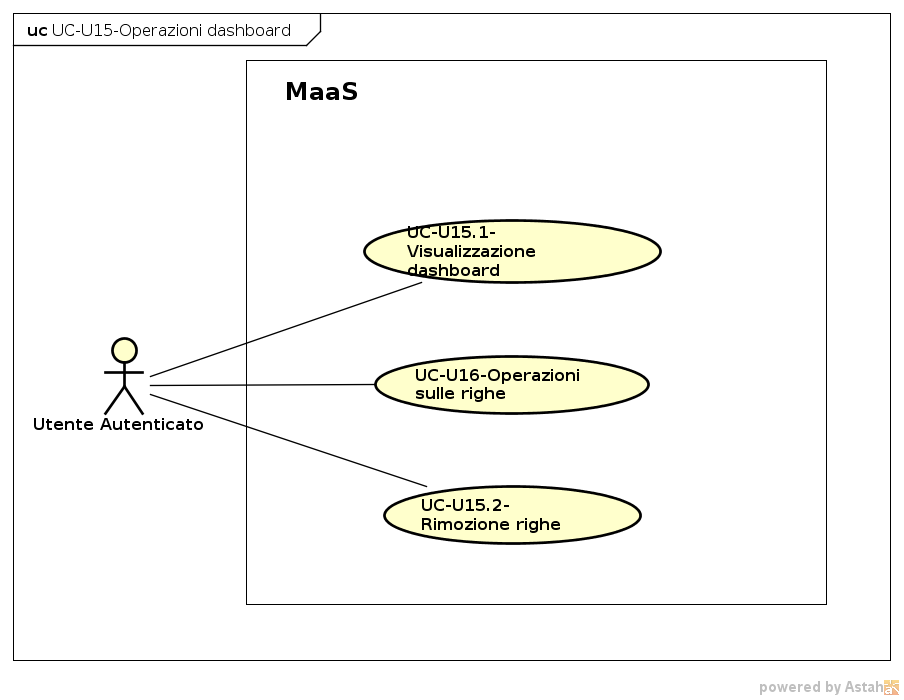
\includegraphics[width=12cm]{res/img/UCUtenti/UCUtenteA/UC-U15-Operazioni-dashboard/UC-U15-Operazioni-dashboard}
      \caption{UC-U15 - Operazioni Dashboard}
      \end{center} 
    \end{figure}

    %Tabella 
    \begin{center}
      \bgroup
      \def\arraystretch{1.8}     
      \begin{longtable}{  p{3.5cm} | p{8cm} } 
        
        \hline
        \multicolumn{2}{ | c | }{ \cellcolor[gray]{0.9} \textbf{UC-U15 - Operazioni Dashboard}} \\ 
        \hline
        
        \textbf{Attori Primari} & Utente autenticato \\ 
        \textbf{Scopo e Descrizione} & L'utente autenticato può: visualizzare la Dashboard, effettuare delle operazioni sulle righe della Dashboard, rimuovere le righe della Dashboard. \\ 
        
        \textbf{Precondizioni}  & L'utente autenticato si trova nella pagina iniziale Dashboard. \\ 
        
        \textbf{Postcondizioni} & L'applicazione MaaS ha eseguito le operazioni richieste dall'utente. \\ 
        \textbf{Flusso Principale} & 1. L'utente autenticato visualizza la Dashboard (UC-U15.1)
        
2. L'utente autenticato effettua delle operazioni sulle righe (UC-U16)

3. L'utente autenticato rimuove delle righe dalla Dashboard (UC-U15.2) \\
        \textbf{Estensioni} & Nessuna \\
        \textbf{Inclusioni} & Nessuna
      \end{longtable}
      \egroup
    \end{center}

\subsubsection{UC-U15.1}

    %Tabella 
    \begin{center}
      \bgroup
      \def\arraystretch{1.8}     
      \begin{longtable}{  p{3.5cm} | p{8cm} } 
        
        \hline
        \multicolumn{2}{ | c | }{ \cellcolor[gray]{0.9} \textbf{UC-U15.1 - Visualizzazione Dashboard}} \\ 
        \hline
        
        \textbf{Attori Primari} & Utente autenticato \\ 
        \textbf{Scopo e Descrizione} & L'utente autenticato visualizza la Dashboard nella pagina Dashboard. \\ 
        
        \textbf{Precondizioni}  & L'utente si trova nella pagina Dashboard. \\ 
        
        \textbf{Postcondizioni} & L'utente ha visualizzato la propria Dashboard. \\ 
        \textbf{Flusso Principale} & Nessuno \\
        \textbf{Estensioni} & Nessuna \\
        \textbf{Inclusioni} & Nessuna
      \end{longtable}
      \egroup
    \end{center}
    
\subsubsection{UC-U15.2}

    %Tabella 
    \begin{center}
      \bgroup
      \def\arraystretch{1.8}     
      \begin{longtable}{  p{3.5cm} | p{8cm} } 
        
        \hline
        \multicolumn{2}{ | c | }{ \cellcolor[gray]{0.9} \textbf{UC-U15.2 - Rimozione righe}} \\ 
        \hline
        
        \textbf{Attori Primari} & Utente autenticato \\ 
        \textbf{Scopo e Descrizione} & L'utente autenticato vuole eliminare delle righe presenti nella sua Dashboard. \\ 
        
        \textbf{Precondizioni}  & L'utente si trova nella pagina Dashboard e seleziona la riga che vuole eliminare. \\ 
        
        \textbf{Postcondizioni} & L'utente visualizzando la Dashboard non visualizza più la riga rimossa. \\ 
        \textbf{Flusso Principale} & Nessuno \\
        \textbf{Estensioni} & Nessuna \\
        \textbf{Inclusioni} & Nessuna
      \end{longtable}
      \egroup
    \end{center}

\subsubsection{UC-U16}

    \begin{figure}[H]
      \begin{center}
        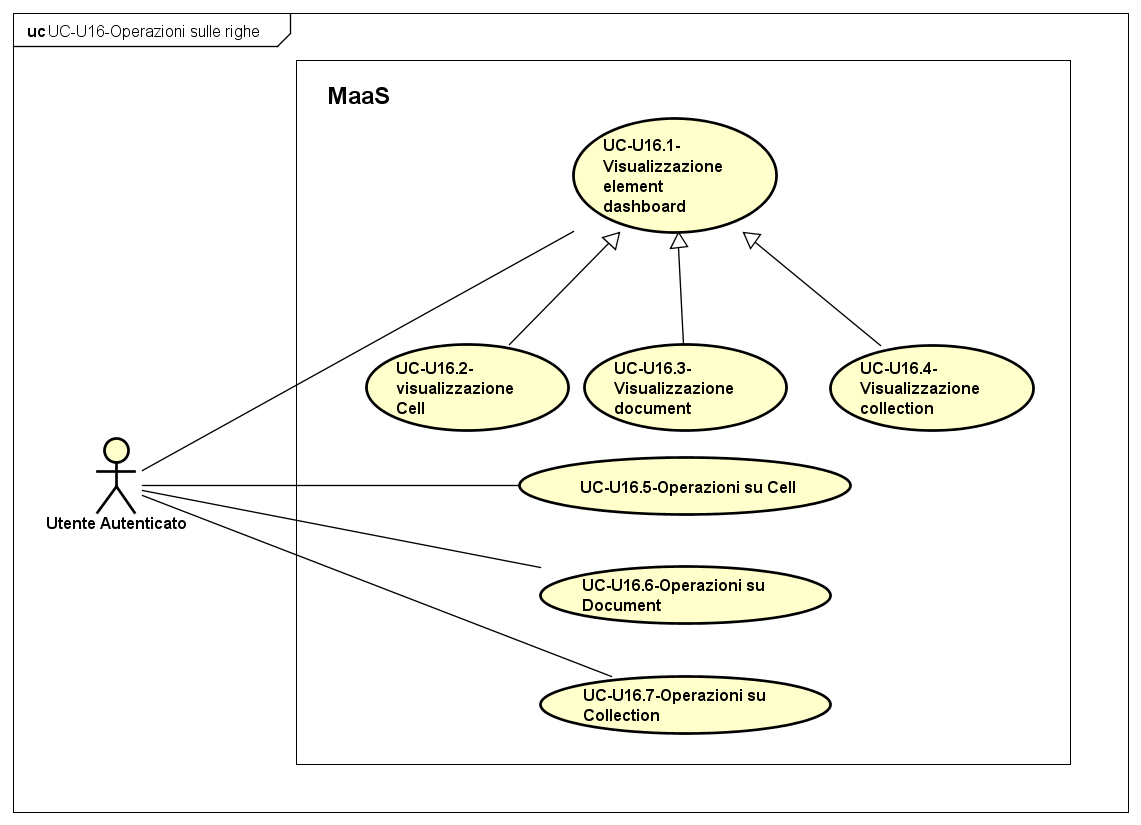
\includegraphics[width=12cm]{res/img/UCUtenti/UCUtenteA/UC-U16-Operazioni_sulle_righe/UC-U16-Operazioni_sulle_righe}
      \caption{UC-U16 - Operazioni sulle righe della Dashboard}
      \end{center} 
    \end{figure}

    %Tabella 
    \begin{center}
      \bgroup
      \def\arraystretch{1.8}     
      \begin{longtable}{  p{3.5cm} | p{8cm} } 
        
        \hline
        \multicolumn{2}{ | c | }{ \cellcolor[gray]{0.9} \textbf{UC-U16 - Operazioni sulle righe della Dashboard}} \\ 
        \hline
        
        \textbf{Attori Primari} & Utente autenticato \\ 
        \textbf{Scopo e Descrizione} & L'utente autenticato può eseguire le seguenti azioni sulle righe della Dashboard: visualizzare un elemento di una riga (che può essere una cell, un document o una collection) oppure effettuare un'operazione su un elemento di una riga. \\ 
        
        \textbf{Precondizioni}  & L'utente autenticato ha visualizzato la pagina iniziale Dashboard. \\ 
        
        \textbf{Postcondizioni} & L'applicazione MaaS ha eseguito le operazioni sulle righe della Dashboard richieste dall'utente autenticato. \\ 
        \textbf{Flusso Principale} & 1. Visualizzazione element Dashboard (UC-U16.1)
        
1.1 L'utente visualizza una cell (UC-U16.2)

1.2 L'utente visualizza un document (UC-U16.3)

1.3 L'utente visualizza una collection (UC-U16.4)

2. L'utente desidera effettuare un'operazione su una riga

2.1 L'utente effettua un'operazione su una cell (UC-U16.5)

2.2 L'utente effettua un'operazione su un document (UC-U16.6)

2.3 L'utente effettua un'operazione su una collection (UC-U16.7) \\
        \textbf{Estensioni} & Nessuna \\
        \textbf{Inclusioni} & Nessuna
      \end{longtable}
      \egroup
    \end{center}
    
\subsubsection{UC-U16.1}

    %Tabella 
    \begin{center}
      \bgroup
      \def\arraystretch{1.8}     
      \begin{longtable}{  p{3.5cm} | p{8cm} } 
        
        \hline
        \multicolumn{2}{ | c | }{ \cellcolor[gray]{0.9} \textbf{UC-U16.1 - Visualizzazione element Dashboard}} \\ 
        \hline
        
        \textbf{Attori Primari} & Utente autenticato \\ 
        \textbf{Scopo e Descrizione} & L'utente autenticato sceglie di visualizzare un element da una riga della Dashboard (che può essere una cell, un document o una collection). \\ 
        
        \textbf{Precondizioni}  & L'utente autenticato ha visualizzato un element della Dashboard. \\ 
        
        \textbf{Postcondizioni} & L'utente autenticato ha visualizzato un element di una riga della Dashboard. \\ 
        \textbf{Flusso Principale} & Nessuno \\
        \textbf{Estensioni} & Nessuna \\
        \textbf{Inclusioni} & Nessuna
      \end{longtable}
      \egroup
    \end{center}

\newpage

\subsubsection{UC-U16.2}

    %Tabella 
    \begin{center}
      \bgroup
      \def\arraystretch{1.8}     
      \begin{longtable}{  p{3.5cm} | p{8cm} } 
        
        \hline
        \multicolumn{2}{ | c | }{ \cellcolor[gray]{0.9} \textbf{UC-U16.2 - Visualizzazione cell}} \\ 
        \hline
        
        \textbf{Attori Primari} & Utente autenticato \\ 
        \textbf{Scopo e Descrizione} & L'utente autenticato può visualizzare una cell selezionandola da una riga della Dashboard. \\ 
        
        \textbf{Precondizioni}  & L'utente autenticato ha visualizzato la pagina Dashboard. \\ 
        
        \textbf{Postcondizioni} & L'utente autenticato è stato reindirizzato nella pagina cell e ne ha visualizzato il contenuto. \\ 
        \textbf{Flusso Principale} & Nessuno \\
        \textbf{Estensioni} & Nessuna \\
        \textbf{Inclusioni} & Nessuna
      \end{longtable}
      \egroup
    \end{center}
    
\subsubsection{UC-U16.3}

    %Tabella 
    \begin{center}
      \bgroup
      \def\arraystretch{1.8}     
      \begin{longtable}{  p{3.5cm} | p{8cm} } 
        
        \hline
        \multicolumn{2}{ | c | }{ \cellcolor[gray]{0.9} \textbf{UC-U16.3 - Visualizzazione document}} \\ 
        \hline
        
        \textbf{Attori Primari} & Utente autenticato \\ 
        \textbf{Scopo e Descrizione} & L'utente autenticato può visualizzare un document selezionandolo da una riga della Dashboard. \\ 
        
        \textbf{Precondizioni}  & L'utente autenticato ha visualizzato la pagina Dashboard. \\ 
        
        \textbf{Postcondizioni} & L'utente autenticato è stato reindirizzato nella pagina document e ne ha visualizzato il contenuto. \\ 
        \textbf{Flusso Principale} & Nessuno \\
        \textbf{Estensioni} & Nessuna \\
        \textbf{Inclusioni} & Nessuna
      \end{longtable}
      \egroup
    \end{center}
    
\subsubsection{UC-U16.4}

    %Tabella 
    \begin{center}
      \bgroup
      \def\arraystretch{1.8}     
      \begin{longtable}{  p{3.5cm} | p{8cm} } 
        
        \hline
        \multicolumn{2}{ | c | }{ \cellcolor[gray]{0.9} \textbf{UC-U16.4 - Visualizzazione collection}} \\ 
        \hline
        
        \textbf{Attori Primari} & Utente autenticato \\ 
        \textbf{Scopo e Descrizione} & L'utente autenticato può visualizzare una collection selezionandola da una riga della Dashboard. \\ 
        
        \textbf{Precondizioni}  & L'utente autenticato ha visualizzato la pagina Dashboard. \\ 
        
        \textbf{Postcondizioni} & L'utente autenticato è stato reindirizzato nella pagina collection e ne ha visualizzato il contenuto. \\ 
        \textbf{Flusso Principale} & Nessuno \\
        \textbf{Estensioni} & Nessuna \\
        \textbf{Inclusioni} & Nessuna
      \end{longtable}
      \egroup
    \end{center}
    
\subsubsection{UC-U16.5}
 

    \begin{figure}[H]
      \begin{center}
        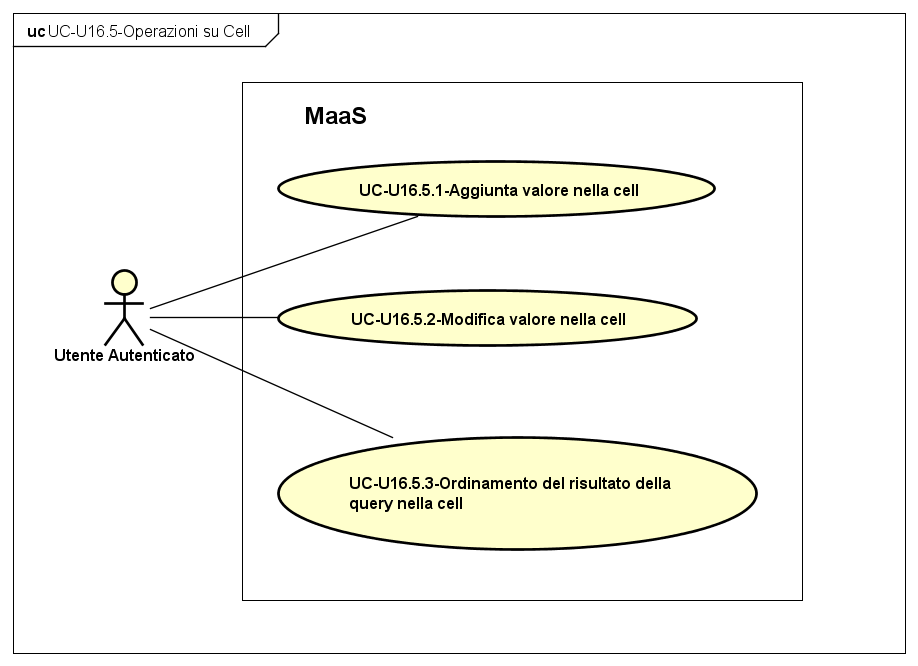
\includegraphics[width=12cm]{res/img/UCUtenti/UCUtenteA/UC-U16.5-Operazioni_su_Cell/UC-U16.5-Operazioni_su_Cell}
      \caption{UC-U16.5 - Operazioni su cell}
      \end{center} 
    \end{figure}

    %Tabella 
    \begin{center}
      \bgroup
      \def\arraystretch{1.8}     
      \begin{longtable}{  p{3.5cm} | p{8cm} } 
        
        \hline
        \multicolumn{2}{ | c | }{ \cellcolor[gray]{0.9} \textbf{UC-U16.5 - Operazioni su cell}} \\ 
        \hline
        
        \textbf{Attori Primari} & Utente autenticato \\ 
        \textbf{Scopo e Descrizione} & L'utente autenticato può eseguire le seguenti operazioni dalla pagina cell: può aggiungere un valore arbitrario, può modificare il valore, può ordinare il valore nella cell in base all'unico campo della query (scritta in un momento precedente nell'editor) che ha prodotto tale valore. \\ 
        
        \textbf{Precondizioni}  & L'utente autenticato ha visualizzato la pagina cell. \\ 
        
        \textbf{Postcondizioni} & L'applicazione MaaS ha eseguito le operazioni richieste dall'utente autenticato. \\ 
        \textbf{Flusso Principale} & 1. L'utente autenticato aggiunge un valore arbitrario nella cell (UC-U16.5.1)
        
2. L'utente autenticato modifica il valore nella cell (UC-U16.5.2)

3. L'utente autenticato ordina il valore nella cell (UC-U16.5.3) \\
        \textbf{Estensioni} & Nessuna \\
        \textbf{Inclusioni} & Nessuna
      \end{longtable}
      \egroup
    \end{center}
	
\subsubsection{UC-U16.5.1}

    %Tabella 
    \begin{center}
      \bgroup
      \def\arraystretch{1.8}     
      \begin{longtable}{  p{3.5cm} | p{8cm} } 
        
        \hline
        \multicolumn{2}{ | c | }{ \cellcolor[gray]{0.9} \textbf{UC-U16.5.1 - Aggiunta di un valore nella cell}} \\ 
        \hline
        
        \textbf{Attori Primari} & Utente autenticato \\ 
        \textbf{Scopo e Descrizione} & L'utente autenticato può aggiungere un valore arbitrario nella cell.  \\ 
        
        \textbf{Precondizioni}  & L'utente autenticato ha visualizzato la pagina cell.  \\ 
        
        \textbf{Postcondizioni} & L'utente autenticato ha aggiunto un valore arbitrario nella cell. \\ 
        \textbf{Flusso Principale} & Nessuno \\
        \textbf{Estensioni} & Nessuna \\
        \textbf{Inclusioni} & Nessuna
      \end{longtable}
      \egroup
    \end{center}
    
\subsubsection{UC-U16.5.2}

    %Tabella 
    \begin{center}
      \bgroup
      \def\arraystretch{1.8}     
      \begin{longtable}{  p{3.5cm} | p{8cm} } 
        
        \hline
        \multicolumn{2}{ | c | }{ \cellcolor[gray]{0.9} \textbf{UC-U16.5.2 - Modifica valore cell}} \\ 
        \hline
        
        \textbf{Attori Primari} & Utente autenticato \\ 
        \textbf{Scopo e Descrizione} & L'utente autenticato può modificare il valore della cell. \\ 
        
        \textbf{Precondizioni}  & L'utente autenticato ha visualizzato la pagina cell. \\ 
        
        \textbf{Postcondizioni} & L'utente autenticato ha modificato il valore della cell. \\ 
        \textbf{Flusso Principale} & Nessuno \\
        \textbf{Estensioni} & Nessuna \\
        \textbf{Inclusioni} & Nessuna
      \end{longtable}
      \egroup
    \end{center}
\subsubsection{UC-U16.5.3}

    %Tabella 
    \begin{center}
      \bgroup
      \def\arraystretch{1.8}     
      \begin{longtable}{  p{3.5cm} | p{8cm} } 
        
        \hline
        \multicolumn{2}{ | c | }{ \cellcolor[gray]{0.9} \textbf{UC-U16.5.3 - Ordinamento cell}} \\ 
        \hline
        
        \textbf{Attori Primari} & Utente autenticato \\ 
        \textbf{Scopo e Descrizione} & L'utente autenticato può ordinare il valore nella cell in base all'unico campo della query (scritta in un momento precedente nell'editor) che ha prodotto tale valore. \\ 
        
        \textbf{Precondizioni}  & L'utente autenticato ha visualizzato la pagina cell. \\ 
        
        \textbf{Postcondizioni} & L'utente autenticato ha ordinato il valore della cell. \\ 
        \textbf{Flusso Principale} & Nessuno \\
        \textbf{Estensioni} & Nessuna \\
        \textbf{Inclusioni} & Nessuna
      \end{longtable}
      \egroup
    \end{center}

\subsubsection{UC-U16.6}
 

    \begin{figure}[H]
      \begin{center}
        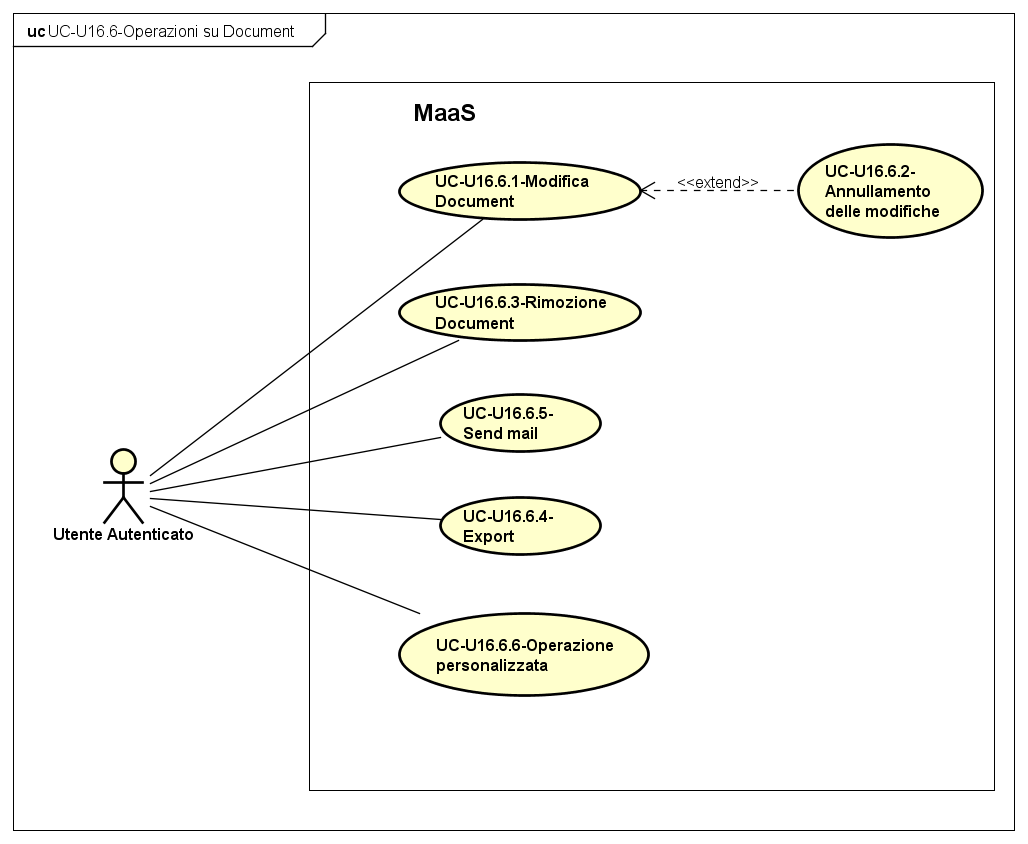
\includegraphics[width=12cm]{res/img/UCUtenti/UCUtenteA/UC-U16.6-Operazioni_su_Document/UC-U16.6-Operazioni_su_Document}
      \caption{UC-U16.6 - Operazioni su document}
      \end{center} 
    \end{figure}

    %Tabella 
    \begin{center}
      \bgroup
      \def\arraystretch{1.8}     
      \begin{longtable}{  p{3.5cm} | p{8cm} } 
        
        \hline
        \multicolumn{2}{ | c | }{ \cellcolor[gray]{0.9} \textbf{UC-U16.6 - Operazioni su document}} \\ 
        \hline
        
        \textbf{Attori Primari} & Utente autenticato \\ 
        \textbf{Scopo e Descrizione} & L'utente autenticato può effettuare le seguenti operazioni dalla pagina document: modificare un document, rimuovere un document, eseguire un'azione di default ("Export" o "send mail") oppure un'azione personalizzata. \\ 
        
        \textbf{Precondizioni}  & L'utente autenticato ha visualizzato la pagina document. \\ 
        
        \textbf{Postcondizioni} & L'applicazione MaaS ha eseguito le operazioni richieste dall'utente autenticato. \\ 
        \textbf{Flusso Principale} & 1. L'utente autenticato modifica un document (UC-U16.6.1)
2. L'utente autenticato rimuove un document (UC-U16.6.3)

3. L'utente autenticato esporta il json e il csv di un document (UC-U16.6.4)

4. L'utente autenticato invia una mail a un altro utente (UC-U16.6.5)

5. L'utente autenticato esegue un'azione personalizzata (UC-U16.6.6) \\
        \textbf{Estensioni} & 1. L'utente desidera annullare le modifiche apportate a un document (UC-U16.6.2) \\
        \textbf{Inclusioni} & Nessuna
      \end{longtable}
      \egroup
    \end{center}
    
\subsubsection{UC-U16.6.1}

    %Tabella 
    \begin{center}
      \bgroup
      \def\arraystretch{1.8}     
      \begin{longtable}{  p{3.5cm} | p{8cm} } 
        
        \hline
        \multicolumn{2}{ | c | }{ \cellcolor[gray]{0.9} \textbf{UC-U16.6.1 - Modifica document}} \\ 
        \hline
        
        \textbf{Attori Primari} & Utente autenticato \\ 
        \textbf{Scopo e Descrizione} & L'utente autenticato può modificare un document (modifica il valore di uno dei campi visualizzati nella pagina document selezionata). \\ 
        
        \textbf{Precondizioni}  & L'utente autenticato ha visualizzato una pagina document all'interno della quale desidera apportare delle modifiche. \\ 
        
        \textbf{Postcondizioni} & L'applicazione MaaS ha apportato le modifiche richieste dall'utente al document selezionato. \\ 
        \textbf{Flusso Principale} & Nessuno \\
        \textbf{Estensioni} & Nessuna \\
        \textbf{Inclusioni} & Nessuna
      \end{longtable}
      \egroup
    \end{center}

\subsubsection{UC-U16.6.3}

    %Tabella 
    \begin{center}
      \bgroup
      \def\arraystretch{1.8}     
      \begin{longtable}{  p{3.5cm} | p{8cm} } 
        
        \hline
        \multicolumn{2}{ | c | }{ \cellcolor[gray]{0.9} \textbf{UC-U16.6.3 - Rimozione document}} \\ 
        \hline
        
        \textbf{Attori Primari} & Utente autenticato \\ 
        \textbf{Scopo e Descrizione} & L'utente autenticato può rimuovere un document dalla Dashboard. \\ 
        
        \textbf{Precondizioni}  & L'utente autenticato ha visualizzato la pagina document da rimuovere. \\ 
        
        \textbf{Postcondizioni} & La pagina document selezionata è stata rimossa. \\ 
        \textbf{Flusso Principale} & Nessuno \\
        \textbf{Estensioni} & Nessuna \\
        \textbf{Inclusioni} & Nessuna
      \end{longtable}
      \egroup
    \end{center}
    
\subsubsection{UC-U16.6.4}

    %Tabella 
    \begin{center}
      \bgroup
      \def\arraystretch{1.8}     
      \begin{longtable}{  p{3.5cm} | p{8cm} } 
        
        \hline
        \multicolumn{2}{ | c | }{ \cellcolor[gray]{0.9} \textbf{UC-U16.6.4 - Azione di default - Export}} \\ 
        \hline
        
        \textbf{Attori Primari} & Utente autenticato \\ 
        \textbf{Scopo e Descrizione} & L'utente autenticato può esportare i file json e csv del document corrente. \\ 
        
        \textbf{Precondizioni}  & L'utente ha visualizzato la pagina del document su cui effettuare l'azione di default export. \\ 
        
        \textbf{Postcondizioni} & L'applicazione MaaS ha eseguito la richiesta dell'utente. \\ 
        \textbf{Flusso Principale} & Nessuno \\
        \textbf{Estensioni} & Nessuna \\
        \textbf{Inclusioni} & Nessuna
      \end{longtable}
      \egroup
    \end{center}
    
\subsubsection{UC-U16.6.5}

    %Tabella 
    \begin{center}
      \bgroup
      \def\arraystretch{1.8}     
      \begin{longtable}{  p{3.5cm} | p{8cm} } 
        
        \hline
        \multicolumn{2}{ | c | }{ \cellcolor[gray]{0.9} \textbf{UC-U16.6.5 - Azione di default - Send Mail}} \\ 
        \hline
        
        \textbf{Attori Primari} & Utente autenticato \\ 
        \textbf{Scopo e Descrizione} & L'utente autenticato può inviare una mail a un altro utente di MaaS. \\ 
        
        \textbf{Precondizioni}  & L'utente ha visualizzato la pagina document su cui effettuare l'operazione di default send mail. \\ 
        
        \textbf{Postcondizioni} & L'applicazione MaaS ha inviato la mail. \\ 
        \textbf{Flusso Principale} & Nessuno \\
        \textbf{Estensioni} & Nessuna \\
        \textbf{Inclusioni} & Nessuna
      \end{longtable}
      \egroup
    \end{center}

\subsubsection{UC-U16.6.6}

    %Tabella 
    \begin{center}
      \bgroup
      \def\arraystretch{1.8}     
      \begin{longtable}{  p{3.5cm} | p{8cm} } 
        
        \hline
        \multicolumn{2}{ | c | }{ \cellcolor[gray]{0.9} \textbf{UC-U16.6.6 - Azione personalizzata}} \\ 
        \hline
        
        \textbf{Attori Primari} & Utente autenticato \\ 
        \textbf{Scopo e Descrizione} & L'utente autenticato può eseguire un'azione personalizzata sul document selezionato. \\ 
        
        \textbf{Precondizioni}  & L'utente autenticato ha visualizzato la pagina del document sul quale desidera effettuare un'azione personalizzata disponibile. \\ 
        
        \textbf{Postcondizioni} & L'applicazione MaaS ha eseguito la richiesta dell'utente. \\ 
        \textbf{Flusso Principale} & Nessuno \\
        \textbf{Estensioni} & Nessuna \\
        \textbf{Inclusioni} & Nessuna
      \end{longtable}
      \egroup
    \end{center}
    
\subsubsection{UC-U16.6.2}

    %Tabella 
    \begin{center}
      \bgroup
      \def\arraystretch{1.8}     
      \begin{longtable}{  p{3.5cm} | p{8cm} } 
        
        \hline
        \multicolumn{2}{ | c | }{ \cellcolor[gray]{0.9} \textbf{UC-U16.6.2 - Annullamento delle modifiche di document}} \\ 
        \hline
        
        \textbf{Attori Primari} & Utente autenticato \\ 
        \textbf{Scopo e Descrizione} & L'utente autenticato può annullare le modifiche precedentemente apportate al document selezionato. \\ 
        
        \textbf{Precondizioni}  & L'utente autenticato ha apportato delle modifiche a un document. \\ 
        
        \textbf{Postcondizioni} & Le modifiche apportate dall'utente autenticato al document selezionato sono state annullate. \\ 
        \textbf{Flusso Principale} & Nessuno \\
        \textbf{Estensioni} & Nessuna \\
        \textbf{Inclusioni} & Nessuna
      \end{longtable}
      \egroup
    \end{center}
    
\subsubsection{UC-U16.7}
 

    \begin{figure}[H]
      \begin{center}
        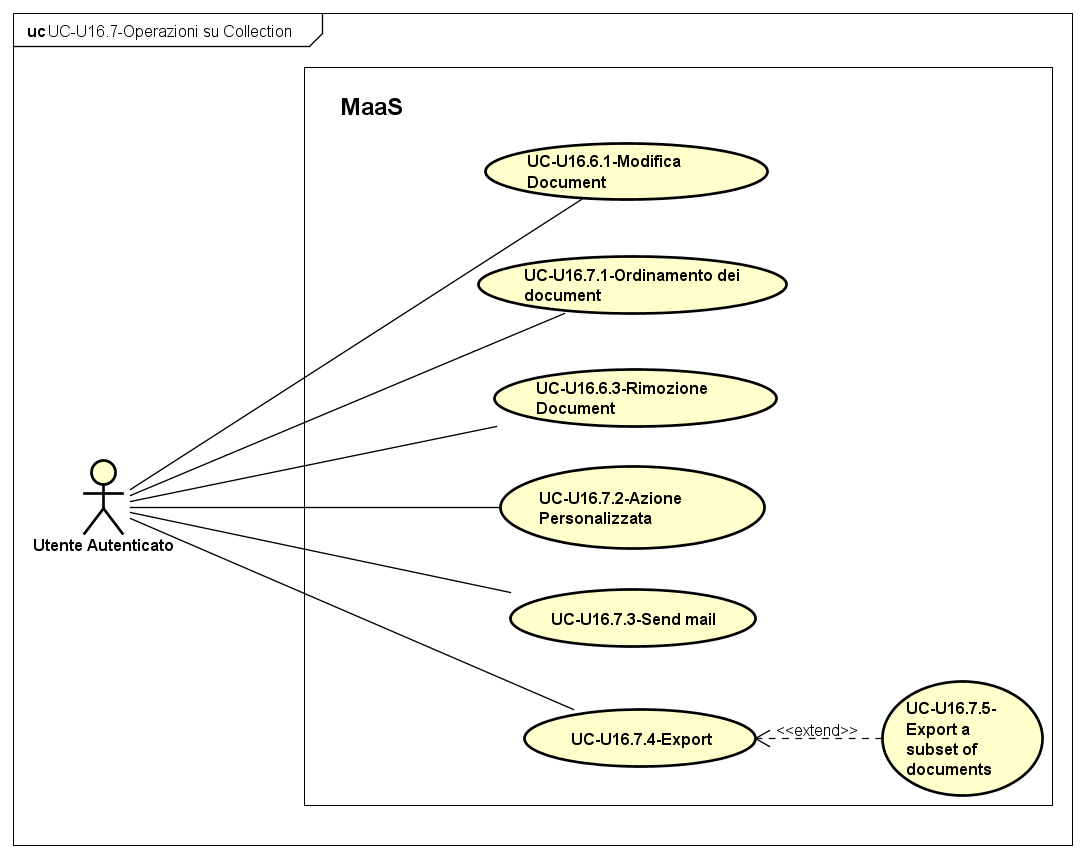
\includegraphics[width=12cm]{res/img/UCUtenti/UCUtenteA/UC-U16.7-Operazioni_su_Collection/UC-U16.7-Operazioni_su_Collection}
      \caption{UC-U16.7 - Operazioni su collection}
      \end{center} 
    \end{figure}

    %Tabella 
    \begin{center}
      \bgroup
      \def\arraystretch{1.8}     
      \begin{longtable}{  p{3.5cm} | p{8cm} } 
        
        \hline
        \multicolumn{2}{ | c | }{ \cellcolor[gray]{0.9} \textbf{UC-U16.7 - Operazioni su collection}} \\ 
        \hline
        
        \textbf{Attori Primari} & Utente autenticato \\ 
        \textbf{Scopo e Descrizione} & L'utente autenticato può eseguire una delle seguenti operazioni su un pagina collection: modificare un document, filtrare i document, selezionare e visualizzare un sottoinsieme di attributi di un sottoinsieme di document, rimuovere un document, eseguire un'azione di default (Export o Send Mail), o un'azione personalizzata. \\ 
        
        \textbf{Precondizioni}  & L'utente autenticato ha visualizzato la pagina collection. \\ 
        
        \textbf{Postcondizioni} & L'applicazione MaaS ha eseguito le operazioni richieste dall'utente autenticato. \\ 
        \textbf{Flusso Principale} & 1. L'utente autenticato può modificare un document (UC-U16.6.1)
        
2. L'utente autenticato può filtrare i document(UC-U16.7.1)

3. L'utente autenticato può selezionare gli attributi da visualizzare dei document(UC-U16.7.2)

4. L'utente autenticato può ordinare i document (UC-U16.7.3)

5. L'utente autenticato può rimuovere un document(UC-U16.6.3)

6. L'utente autenticato può eseguire l'azione di default send mail(UC-U16.7.4)

7. L'utente autenticato può eseguire l'azione di default export(UC-U16.7.5)

8. L'utente autenticato può eseguire un'azione personalizzata(UC-U16.7.6) \\
        \textbf{Estensioni} & 1. L'utente può decidere di selezionare solo un sottoinsieme di elementi per i quali desidera esportare i file .json e .csv (UC-U16.7.6) \\
        \textbf{Inclusioni} & Nessuna
      \end{longtable}
      \egroup
    \end{center}
    
\subsubsection{UC-U17}
      
        %Tabella 
        \begin{center}
          \bgroup
          \def\arraystretch{1.8}     
          \begin{longtable}{  p{3.5cm} | p{8cm} } 
            
            \hline
            \multicolumn{2}{ | c | }{ \cellcolor[gray]{0.9} \textbf{UC-U17 - Logout}} \\ 
            \hline
            
            \textbf{Attori Primari} & Utente autenticato \\ 
            \textbf{Scopo e Descrizione} & L’utente autenticato vuole effettuare il logout da MaaS.\\ 
            
            \textbf{Precondizioni}  & L'utente autenticato è loggato con le sue credenziali su MaaS. \\ 
            
            \textbf{Postcondizioni} & L'utente autenticato visualizza un messaggio di avvenuto logout e viene disconnesso da MaaS. \\ 
            \textbf{Flusso Principale} & Nessuno \\
            \textbf{Estensioni} & Nessuna  \\
            \textbf{Inclusioni} & Nessuna
          \end{longtable}
          \egroup
        \end{center}
\newpage